    \documentclass[12pt,a4paper]{article}
    \usepackage[T2A]{fontenc}
    \usepackage[utf8]{inputenc}
    \usepackage[russian]{babel}
    \usepackage{amsmath}
    \usepackage{amssymb}
    \usepackage{graphicx}
    \usepackage{floatrow}
    \usepackage{booktabs}
    \usepackage{wrapfig}
    \usepackage{lipsum}
    \usepackage{subcaption}
    \usepackage{fancyhdr}
    \usepackage{mathrsfs}
    \usepackage{tikz}

    \usepackage{graphicx, scalerel}
    \usepackage[warn]{mathtext}
    \usepackage{indentfirst}
    \usepackage[margin = 25mm]{geometry}
    \usepackage{caption}
    \usepackage{multirow}
    \usepackage{gensymb}
    
    \newcommand{\figref}[1]{(См. рис. \ref{#1})}
    \newcommand{\secref}[1]{(См. раздел. \ref{#1})}
    
    \newcommand{\e}[1]{\text{$\cdot10^{#1}$}}
    
    \pagestyle{fancy}
    \fancyhead{}
    \fancyhead[L]{Работа 5.4.2}
    \fancyhead[R]{}
    \fancyfoot[C]{\thepage}
    
    \author{\normalsize Выполнил: Голубович Тимур, группа Б01-110 \\
    	\normalsize 20.09.2023}
    \date{}

    \usepackage{float}
    \restylefloat{table}
    \title{
    	\large Отчет о выполнении лабораторной работы 5.4.2 \\
    	\Large Изучение энергетического спектра $\beta$-частиц и определение их максимальной энергии при помощи магнитного спектрометра
     }

    \begin{document}
    	\maketitle

    \section*{Цель работы}

    С помощью магнитного спектрометра исследовать энергетический спектр $\beta$-частиц при распаде ядер $^{137}$Cs и определить их максимальную энергию.

    \section*{Оборудование и приборы}

    Магнитный спектрометр с "короткой линзой"; высоковольтный и низковольтный выпрямители; форвакуумный насос и вакууметр; ЭВМ.
	
    \section*{Теоретическое введение}

    Бета-распадом называется самопроизвольное превращение ядер, при котором их массовое число не изменяется, а заряд увеличивается или уменьшается на единицу. Бета-активные ядра встречаются во всей области значений массового числа $A$, начиная от единицы (свободный нейтрон) и кончая самыми тяжелыми ядрами.	

	В данной работе мы будем иметь дело с электронным распадом

	\begin{equation*}
		_Z^A\text{X} \; \longrightarrow \;\; _{Z+1}^{\;\;\;\;\,A}\text{X} + e^- + \widetilde{\nu},
	\end{equation*}

	\noindent при котором кроме электрона испускается антинейтрино. Освобождающаяся при $\beta$-распаде энергия делится между электроном, антинейтрино и дочерним ядром, однако доля энергии, передаваемой ядру, исчезающе мала по сравнению с энергией, уносимой электроном и антинейтрино. Практически можно считать, что эти две частицы делят между собой всю освобождающуюся энергию. Поэтому электроны могут иметь любое значение энергии — от нулевой до некоторой максимальной, которая равна энергии, освобождающейся при $\beta$-распаде, являющейся важной физической величиной.
	
	Кинетическая энергия электрона $E$ связана с его импульсом обычным релятивистским соотношением
	\begin{equation}
		E = \sqrt{(pc)^2 + (mc^2)^2} - mc^2.
	\end{equation}

	\begin{figure}[h!]
		\centering
		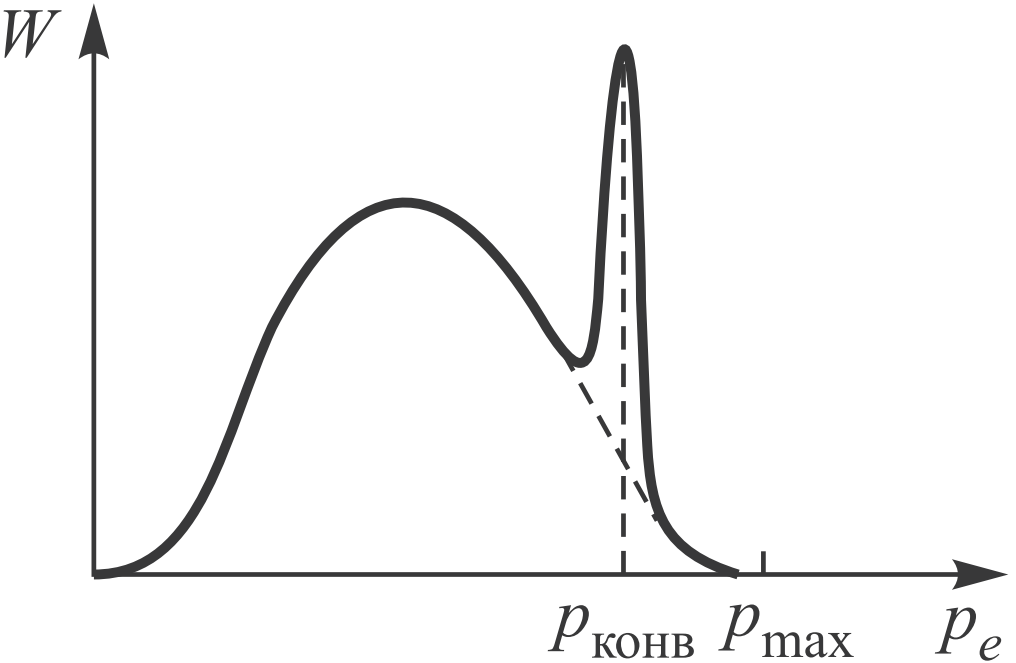
\includegraphics[width=10cm]{res/w_p.png}
		\caption{Форма спектра $\beta$-частиц при разрешенных переходах}
		\label{BetaParticles_Spectre}
	\end{figure}

	В нерелятивистском приближении формула, выражающая форму $\beta$-спектра приобретает вид:
	\begin{equation}
		\frac{dN}{dE} = \sqrt{E}(E_e - E)^2,
		\label{BetaParticles_dNdE}
	\end{equation}

	\noindent где $E_e$ — максимальная энергия электрона.
	
	Выражение (\ref{BetaParticles_dNdE}) приводит к спектру, имеющему вид широкого колокола (см. рис. \ref{BetaParticles_Spectre}). Кривая плавно отходит от нуля и столь же плавно, по параболе, касается оси абсцисс в области максимальной энергии электронов $E_e$.
	
	
	Дочерние ядра, возникающие в результате $\beta$-распада, нередко оказываются возбужденными. Возбужденные ядра отдают свою энергию либо излучая $\gamma$-квант (энергия которого равна разности энергий начального и конечного уровней), либо передавая избыток энергии одному из электронов с внутренних оболочек атома. Излучаемые в таком процессе электроны имеют строго определенную энергию и называются конверсионными.

	Конверсия чаще всего происходит на оболочках $K$ или $L$. На спектре, представленном на рис. \ref{BetaParticles_Spectre}, видна монохроматическая линия, вызванная электронами конверсии. Ширина этой линии в нашем случае является чисто аппаратурной — по ней можно оценить разрешающую силу спектрометра.
	

    \newpage
 
	\section*{Экспериментальная установка}

    \begin{figure}[h!]
		\centering
		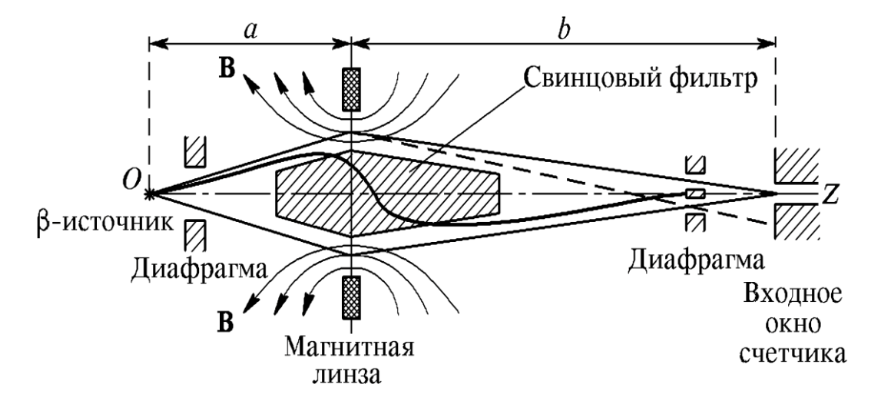
\includegraphics[width=\linewidth]{res/scheme.png}
		\caption{Схема $\beta$-спектрометра с короткой магнитной линзой}
		\label{BetaParticles_Scheme}
	\end{figure}

	Энергию $\beta$-частиц определяют с помощью $\beta$-спектрометров. В работе используется магнитный спектрометр с «короткой линзой». Электроны, испускаемые радиоактивным источником (рис. \ref{BetaParticles_Scheme}), попадают в магнитное поле катушки, ось которой параллельна оси $OZ$ (оси симметрии прибора). Траектории электронов в магнитном поле представляют собой схематически показанные на рисунке сложные спирали, сходящиеся за катушкой в фокусе, расположенном на оси $OZ$. В фокусе установлен детектор электронов. Чувствительным элементом сцинтилляционного счетчика является тонкий кристалл полистирола. При попадании электрона в кристалле возникает световая вспышка -- сцинтилляция, регистрируемая фотоумножителем.
	
	При заданной силе тока на входное окно счетчика фокусируются электроны с определенным импульсом. Электроны, обладающие другими значениями импульса, при этом не сфокусированы и в основном проходят мимо окна (штриховой луч). При изменении тока в катушке на счетчик последовательно фокусируются электроны с разными импульсами. Так как геометрия прибора в течение всего опыта остается неизменной, импульс сфокусированных электронов пропорционален величине тока $I$:
	\begin{equation}
		p_e = kI.
		\label{BetaParticles_pkI}
	\end{equation}

	Из-за конечных размеров источника, диафрагм и окна счетчика, а также вследствие аберраций при заданной величине фокусного расстояния на счетчик попадают электроны с импульсами, лежащими внутри некоторого интервала от $p_e - \Delta p_e/2$ до $p_e + \Delta p_e/2$. Величина $\Delta p_e$ -- ширина интервала импульсов, регистрируемых при заданном значении тока, -- называется разрешающей способностью $\beta$-спектрометра.
	
	Ширина интервала $\Delta p_e$, регистрируемого спектрометром, пропорциональна величине импульса.
	
	В результате попадания электронов в сцинтиллятор на выходе фотоумножителя появляются электрические импульсы, которые заносятся в память персонального компьютера и выводятся на экран монитора. Давление в спектрометре поддерживается на уровне около 0.1 Тор и измеряется термопарным вакуумметром.
	
	
    \section*{Ход работы}
	
    \begin{enumerate}
		\item Откачаем воздух из полости спектрометра.
		
		\item Включим формирователь импульсов, питание магнитной линзы и уменьшим ток через нее до нуля.
		
		\item Приступим к подробному измерению $\beta$-спектра. Результаты запишем в таблицу \ref{BetaParticles_ExpTable}.
		\begin{figure}[h!]
			\centering
			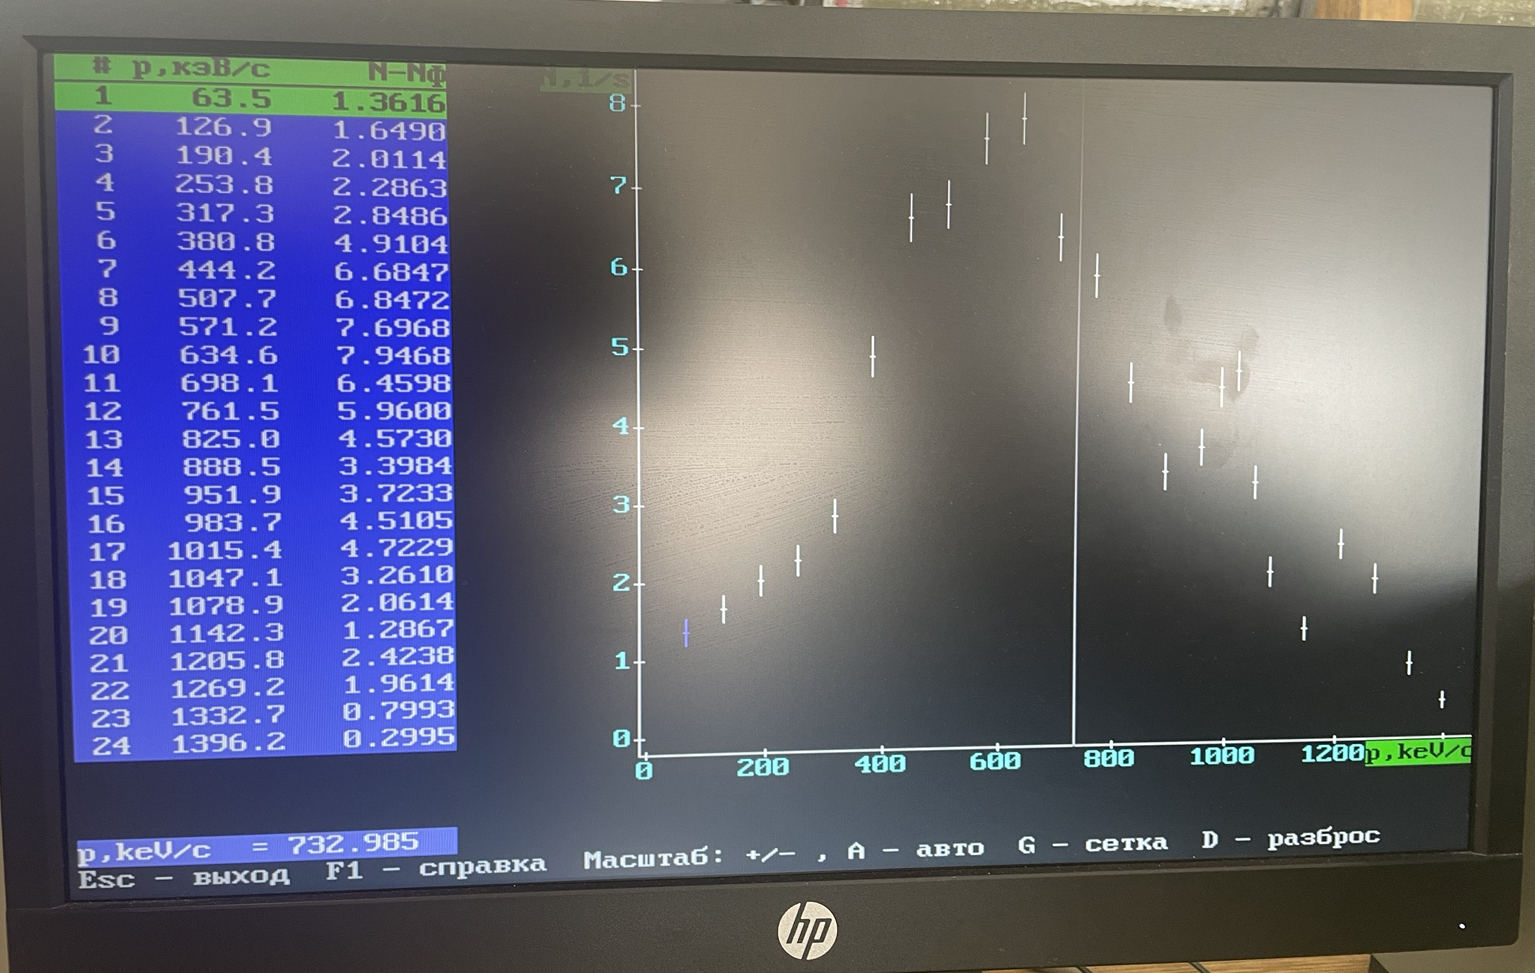
\includegraphics[width=10cm]{src/CompSpectre.jpg}
			\caption{Картина спектра на компьютере}
		\end{figure}
	
		\begin{figure}[h!]
			\centering
			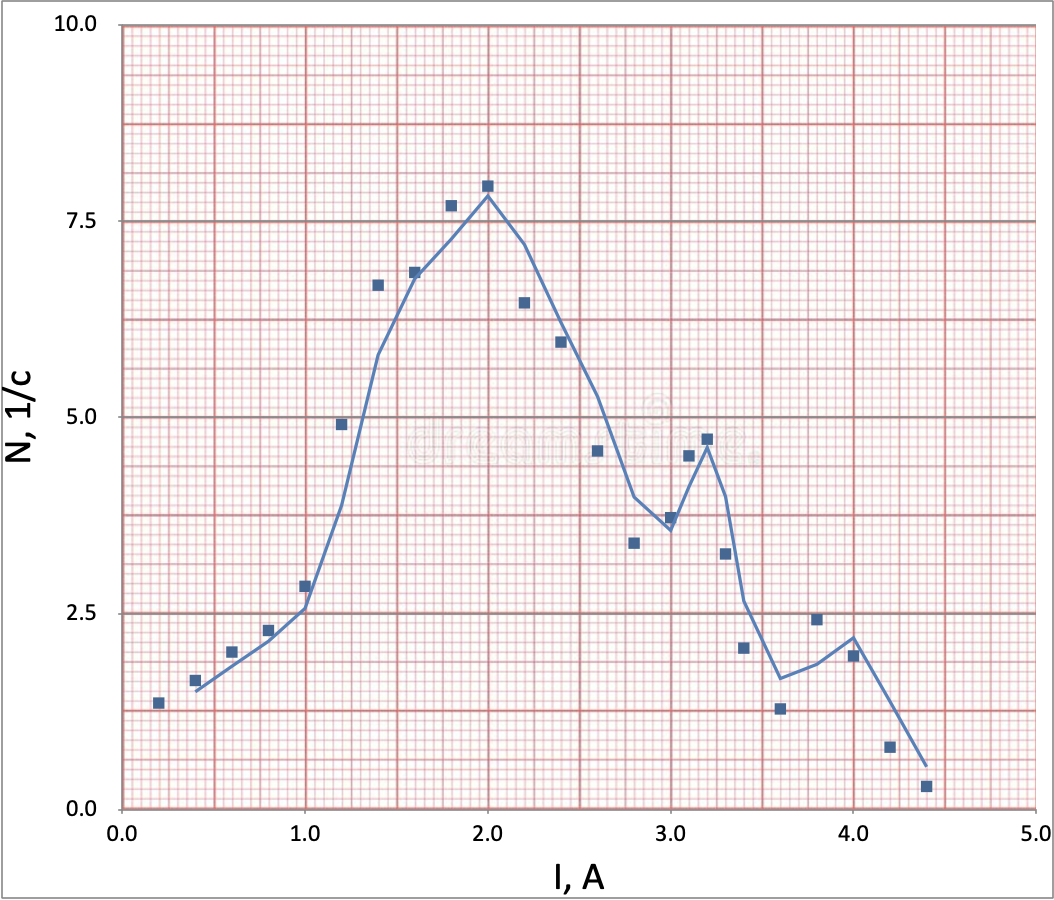
\includegraphics[width=10cm]{src/Spectre.png}
			\caption{$\beta$-спектр за вычетом фона}
		\end{figure}
		
		\item Измерим фон. В нашем случае он получился $N_\text{ф} = 0.929$ с$^{-1}$. Эту информацию тоже занесем в таблицу \ref{BetaParticles_ExpTable}. 


  \begin{table}[h!]
       \centering
       \footnotesize
       \begin{tabular}{cccc}
\toprule
Количество пластин & $l$, см & $N_1$ & $N_2$ \\
\midrule
\multicolumn{4}{c}{Свинец} \\
\midrule
1 & 0.49 & 74415 & 75164 \\
2 & 0.97 & 41098 & 42065 \\
3 & 1.45 & 23371 & 23489 \\
4 & 1.90 & 13985 & 13987 \\
5 & 2.35 & 8452  & 8251  \\
\midrule
\multicolumn{4}{c}{Железо} \\
\midrule
1 & 1.01 & 77976 & 77286 \\
2 & 2.04 & 42158 & 40827 \\
3 & 3.02 & 23599 & 23808 \\
4 & 4.03 & 13315 & 13294 \\
5 & 5.03 & 7667  & 7552  \\
\midrule
\multicolumn{4}{c}{Алюминий} \\
\midrule
1 & 2.01 & 90864 & 89504 \\
2 & 4.02 & 58396 & 58788 \\
3 & 5.99 & 38139 & 38010 \\
4 & 7.99 & 24878 & 24118 \\
5 & 9.98 & 16626 & 16524 \\
\midrule
\multicolumn{4}{c}{Пробки} \\
\midrule
\multicolumn{2}{c}{Количество пробок} & \multicolumn{2}{c}{$N_0$} \\
\midrule
\multicolumn{2}{c}{0} & \multicolumn{2}{c}{139843} \\
\multicolumn{2}{c}{1} & \multicolumn{2}{c}{136826} \\
\multicolumn{2}{c}{2} & \multicolumn{2}{c}{133850} \\
\multicolumn{2}{c}{3} & \multicolumn{2}{c}{131576} \\
\multicolumn{2}{c}{4} & \multicolumn{2}{c}{129176} \\
\bottomrule
\end{tabular}

       \caption{Экспериментальные данные}
       \label{BetaParticles_ExpTable}
    \end{table}

  \item По конверсионному пику определим константу пропорциональности $k$ из уравнения \eqref{BetaParticles_pkI}. Величина произведения импульса конверсионного электрона на скорость света равна 1013.5 кэВ. Откуда:
		\begin{equation*}
			k = 281.5 \cdot \frac{1}{c}\; \frac{\text{кэВ}}{\text{A}},
		\end{equation*}
	 	\noindent где $c$ -- это скорость света, а не секунды.
	 	
	 	\item Теперь, зная эту калибровочную константу, построим график Ферми-Кюри, то есть зависимость величины $\frac{\sqrt{N}}{p^{3/2}}$ от энергии электрона $E$. Из него, по пересечению с осью абсцисс можно определить максимальную энергию $\beta$-частиц.

		\begin{figure}[h!]
			\centering
			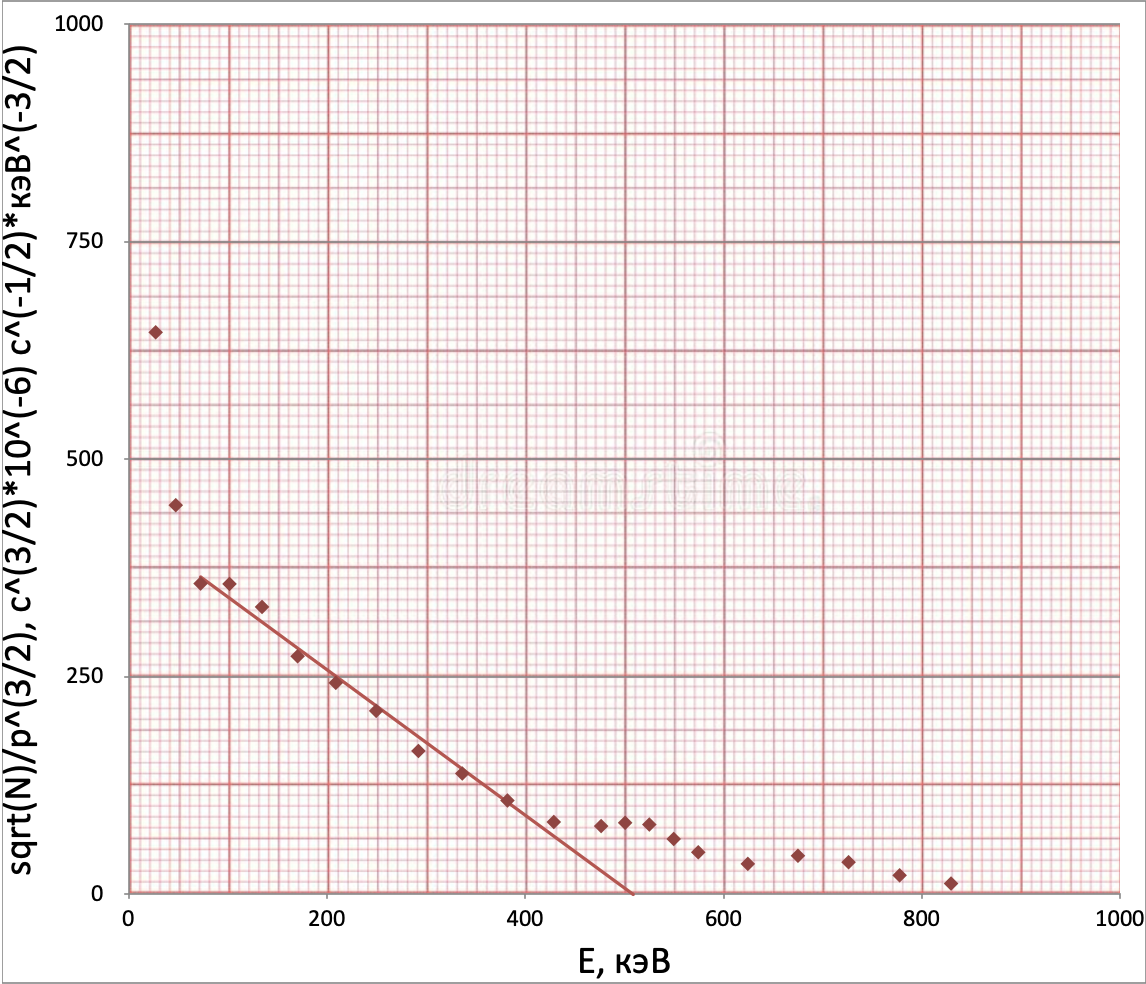
\includegraphics[width=10cm]{src/jopa(E).png}
			\caption{График Ферми-Кюри}
		\end{figure}
	
		Для построения графика не использовались первые 4 точки, поскольку они давали слишком большие значения по ординате из-за чего главную часть графика не было хорошо видно.
		
		Также, мы видим, что сам график хоть и напоминает прямую, однако все же он не линеен. Именно поэтому строим аппроксимирующую прямую лишь по линейному участку.
		
		Получаем следующие коэффициенты для аппроксимации прямой $y = Ax + B$:
		\begin{itemize}
			\item $A = (-0.84 \pm 0.02)$ $c^{3/2} \cdot 10^{-6}$ с$^{-1/2} \cdot$ кэВ$^{-5/2}$
			
			\item $B = (425 \pm 5)$ $c^{3/2} \cdot 10^{-6}$ с$^{-1/2} \cdot$ кэВ$^{-3/2}$
		\end{itemize}
	
		Максимальная энергия $\beta$-частиц определяется пересечением прямой с осью абсцисс:
		\begin{equation*}
			E_\text{max} = -\frac{B}{A}
		\end{equation*}
		\begin{equation*}
			\boxed{E_\text{max} = (509 \pm 30) \text{ кэВ}}
		\end{equation*}
		
		Относительная погрешность составляет $\thicksim 5\%$.
		
		Значение получилось несколько заниженное, по сравнению с табличным: $E_\text{max}^\text{истин} \simeq 634 \text{ кэВ}$.
	\end{enumerate}



	\section*{Вывод}
    	В данной работе мы исследовали спектр $\beta$-частиц при распаде цезия $^{137}$Cs. Также, была определена максимальная энергия $\beta$-частиц при данном распаде: $E_\text{max} = (509 \pm 30)$ кэВ. Относительная погрешность составляет $\thicksim 6\%$. Истинное значение находится немного больше, чем найденное нами: $E_\text{max}^\text{истин} \simeq 634$ кэВ. Хоть ошибки и есть, но достаточно малы.

\newpage
\begin{thebibliography}{9}
	\bibitem{max} \emph{Лабораторный практикум по общей физике. В 3 томах. Том 3. Квантовая физика: учебное пособие} под ред. Ю. М. Ципенюка
\end{thebibliography}

\end{document}
